%%---------------------------------------------------------------------------%%
\section{NekRS: recent developments enabling large scale ExaSMR simulations}
\label{sec:nekrs}


\subsection{Verification of the $\lowercase{k}-\tau$ RANS model in NekRS}
\label{sec:nrs1}
The $k-\tau$ model is implemented in nekRS as the primary RANS model because of two important reasons: (i) its capability in predicting the wall-bounded turbulent flows, and (ii) the relatively easier treatment of boundary conditions. Before conducting the large-scale full core CFD simulations with nekRS, a verification study is performed to ensure the $k-\tau$ model implemented in nekRS produces consistent results as in its CPU-only version, Nek5000. A 2x2 subchannel bundle domain is selected in the testing case. Identical boundary and initial conditions are specified in the nekRS and Nek5000 test cases. The same set of input parameters are given in both cases, such as the time step size, residual tolerances, etc. The cases are run long enough till the steady state. Figure~\ref{fig:tkeofbundle} shows the turbulent kinetic energy distribution under the steady state. A quantitative comparison is presneted in Figure~\ref{fig:tkeplot} and Figure~\ref{fig:tauplot} where the nekRS was able to reproduce the exact solutions of Nek5000. This benchmark study provides a strong footing as we move on to the more extensive  verification and applications of $k-\tau$ model in nekRS.


\begin{figure}[!ht]
\centering
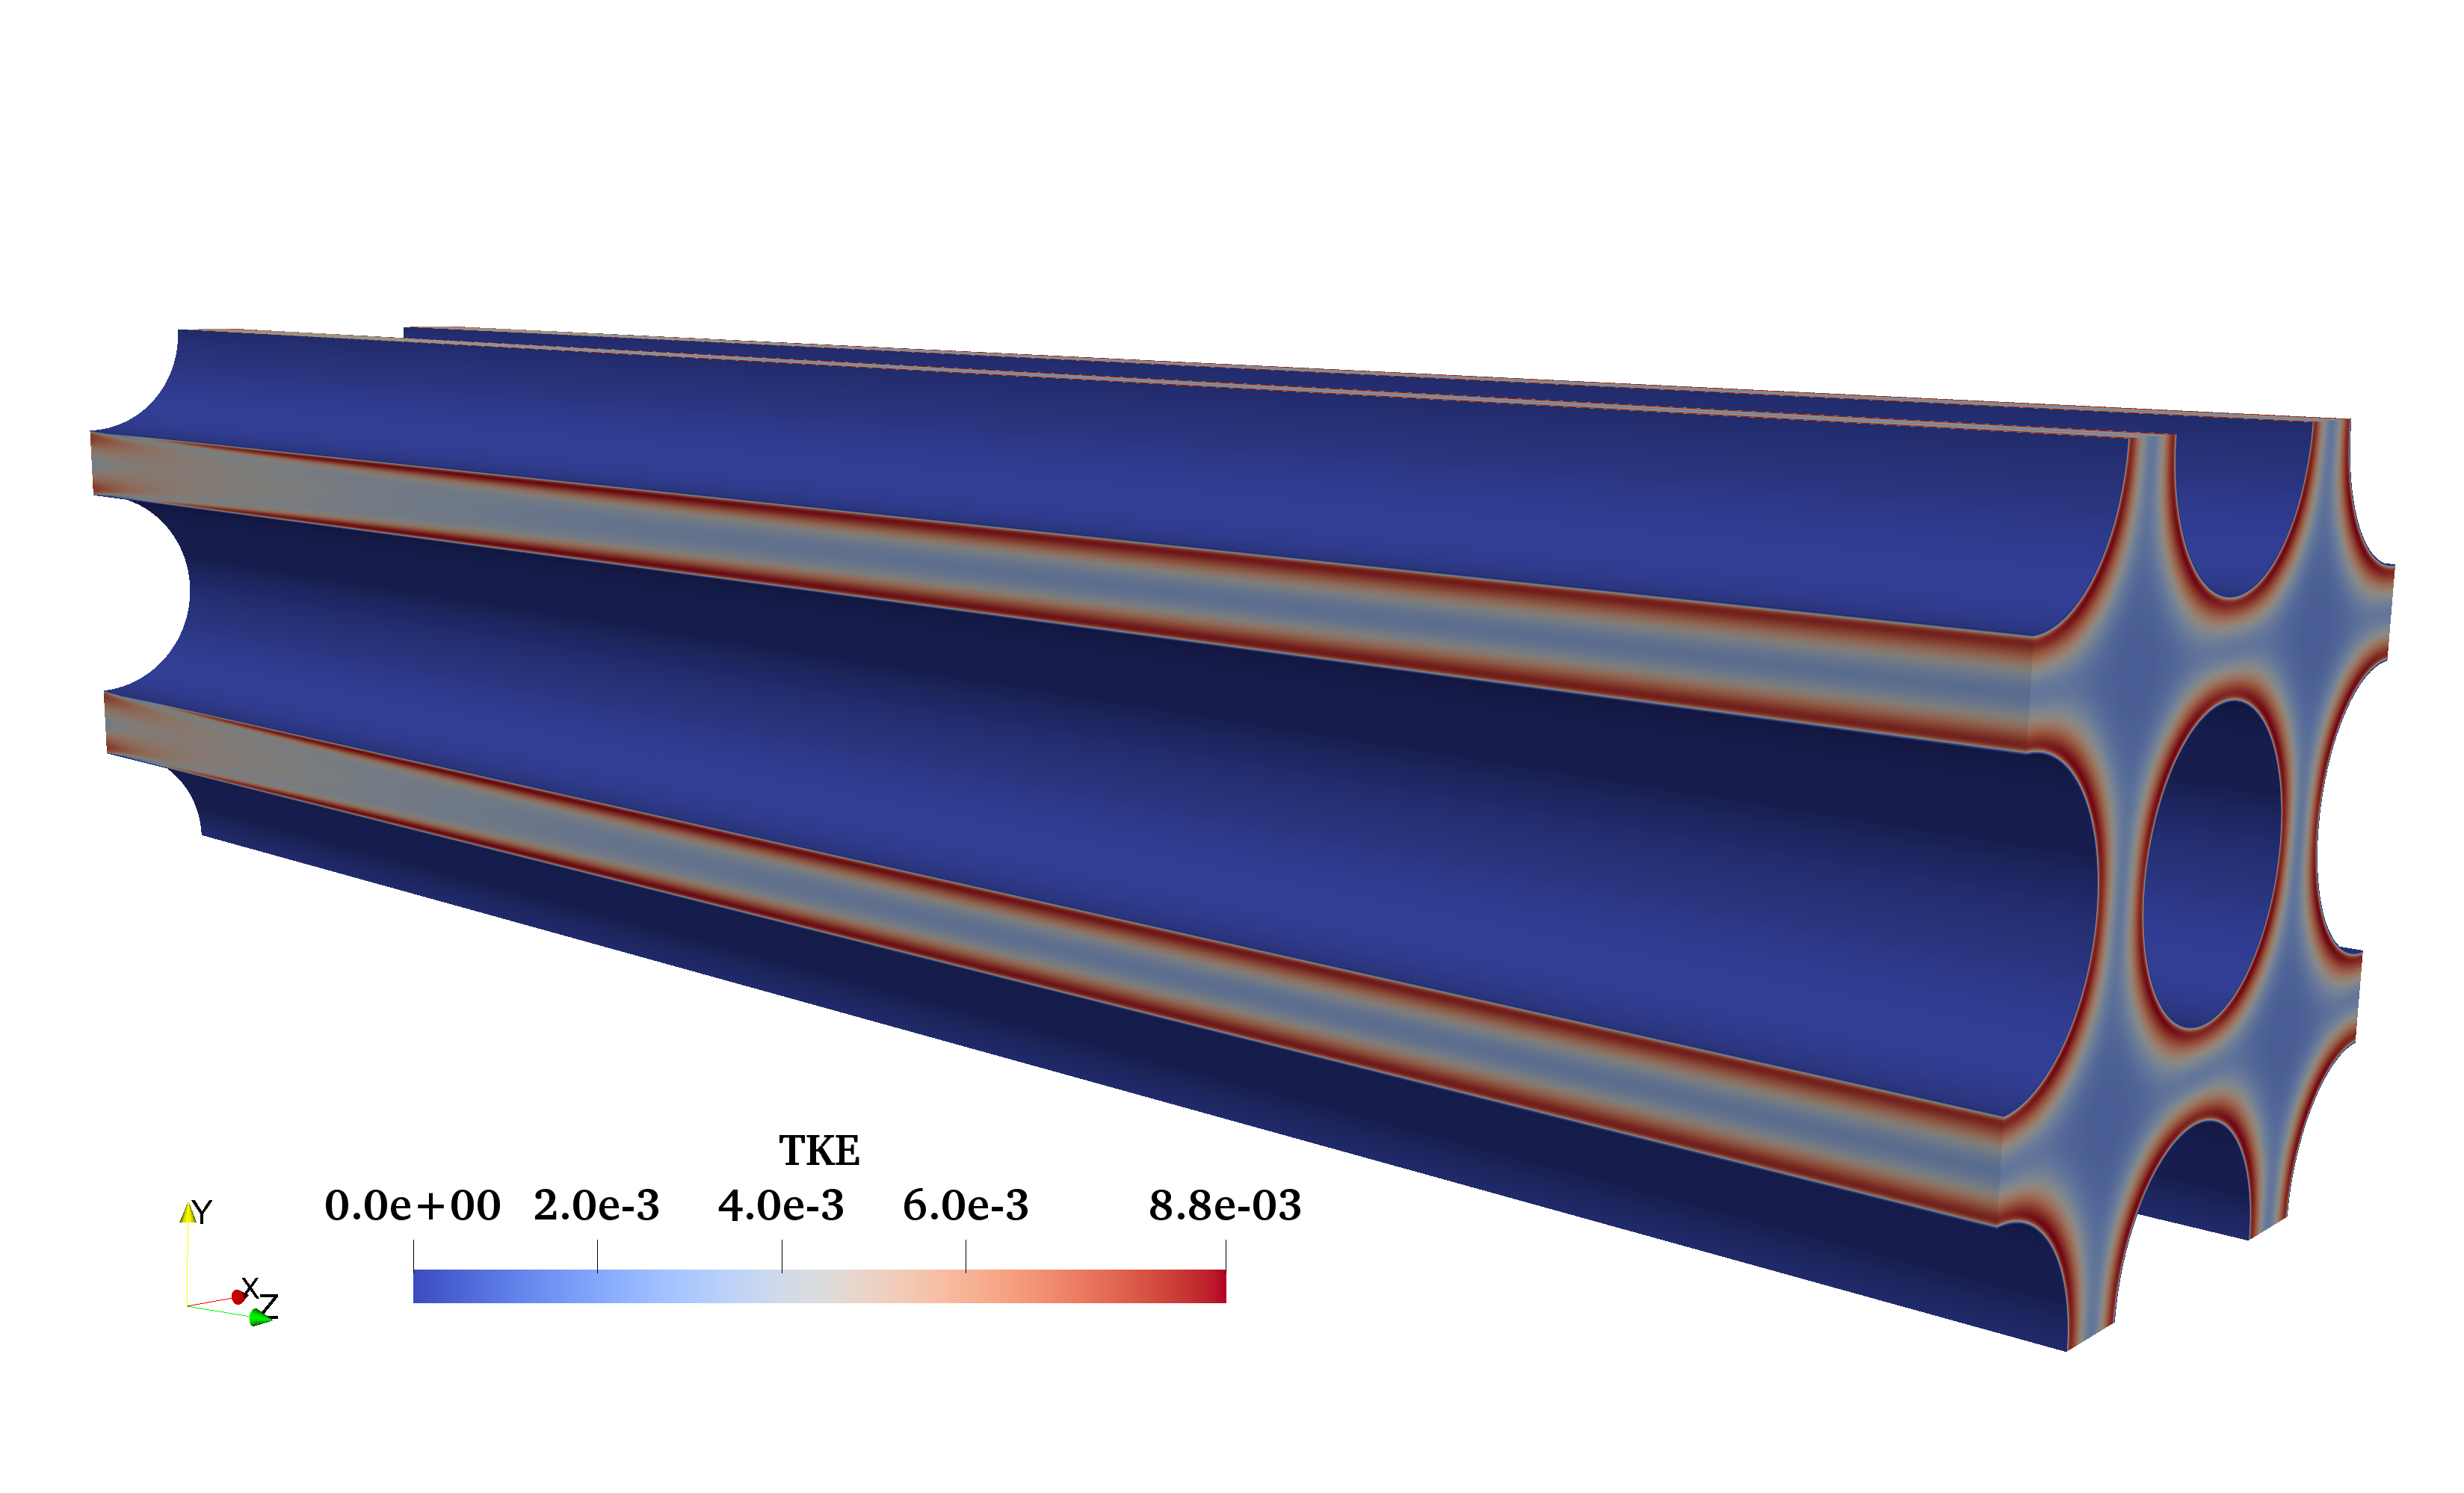
\includegraphics[width=0.5\textwidth]{./figures/TKE_in_bundle.png}
\caption{The steady-state turbulent kinetic energy distribution in the nekRS test case. }
\label{fig:tkeofbundle}
\end{figure}

\begin{figure}[!ht]
\centering
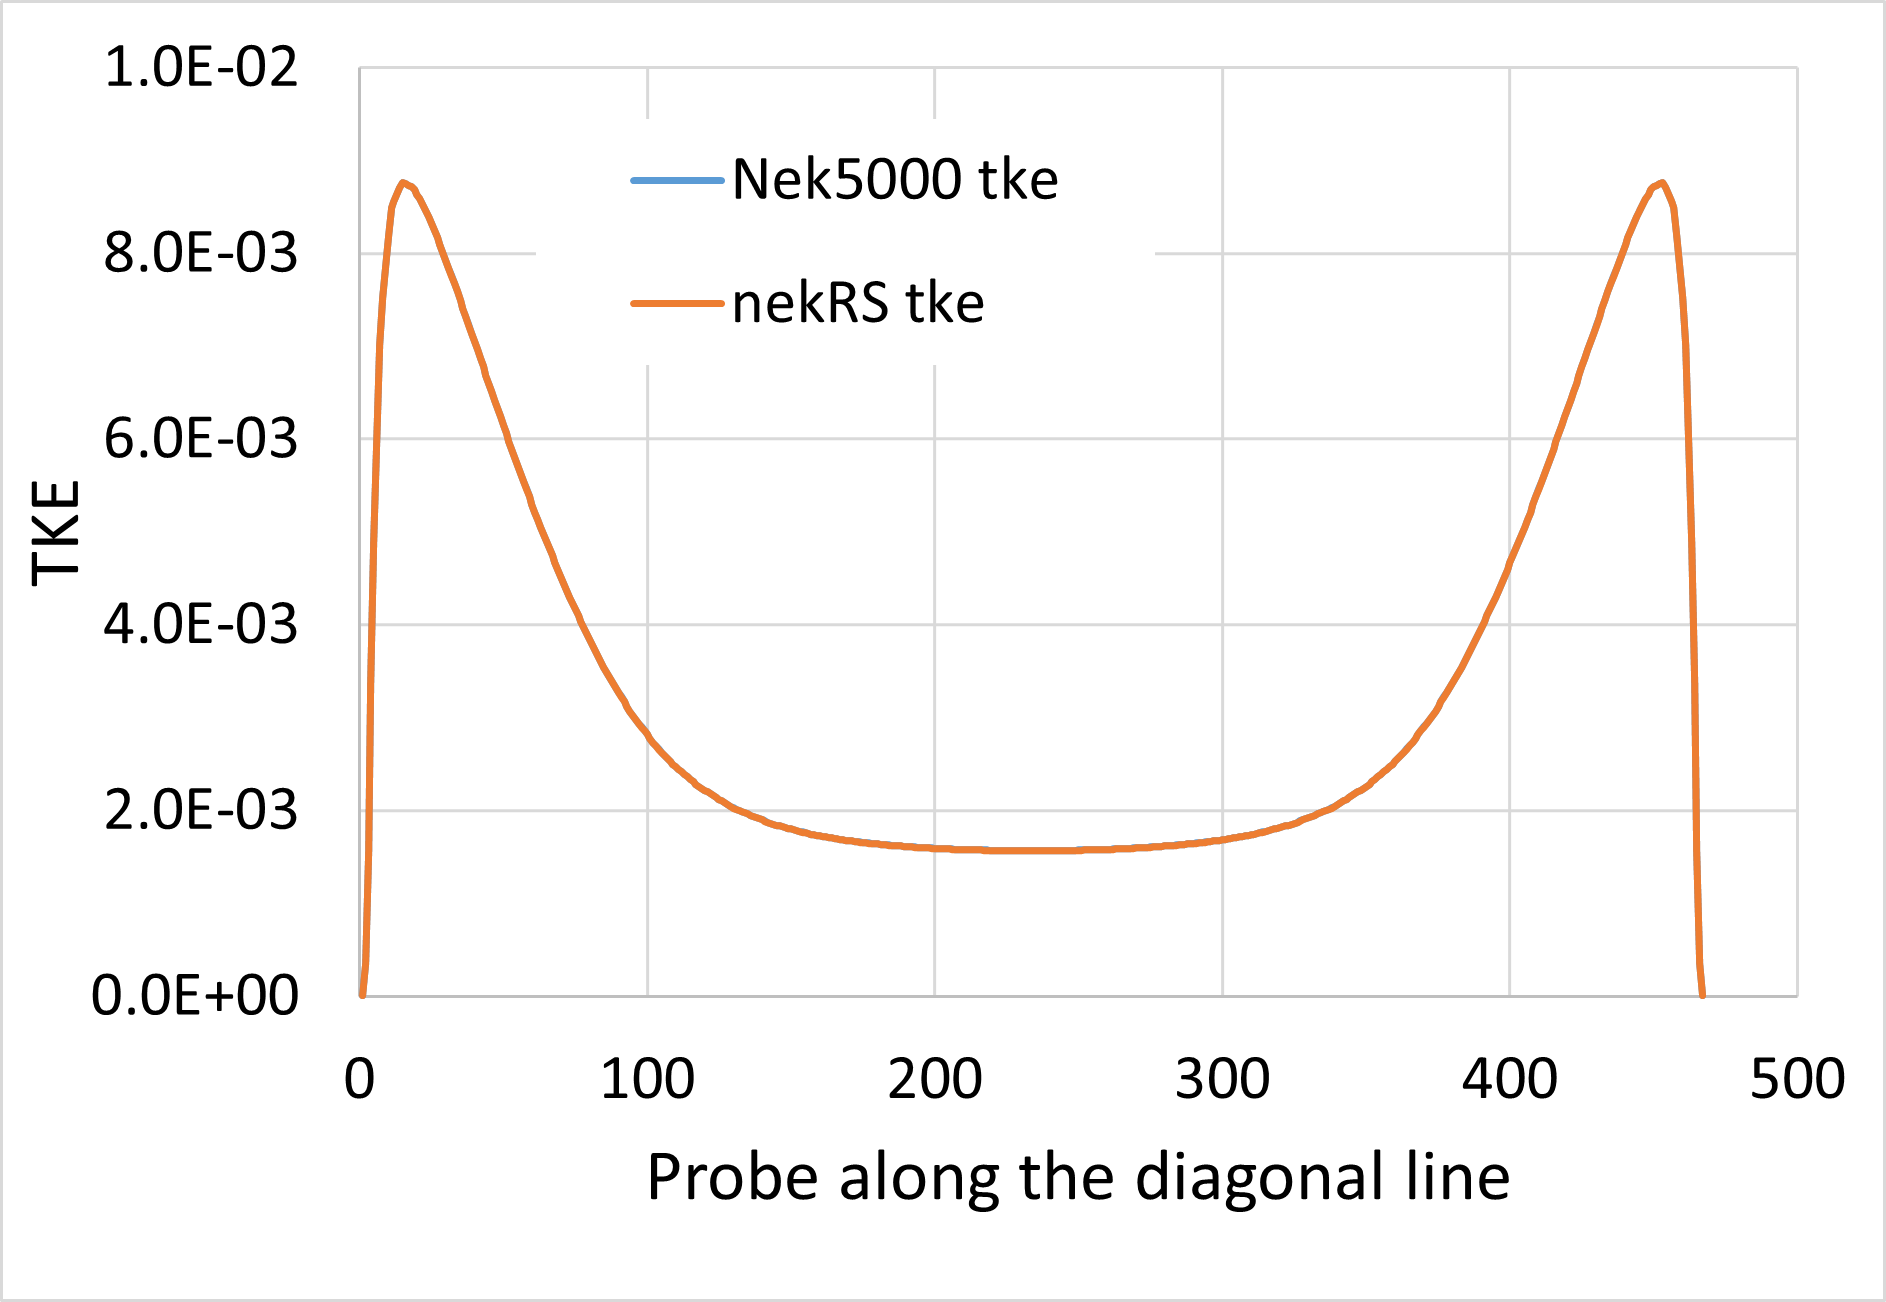
\includegraphics[width=0.5\textwidth]{./figures/tke_verification_bundle2x2.png}
\caption{Comparison of $k$ profile along the outlet diagonal line from Nek5000 and nekRS tests. }
\label{fig:tkeplot}
\end{figure}

\begin{figure}[!ht]
\centering
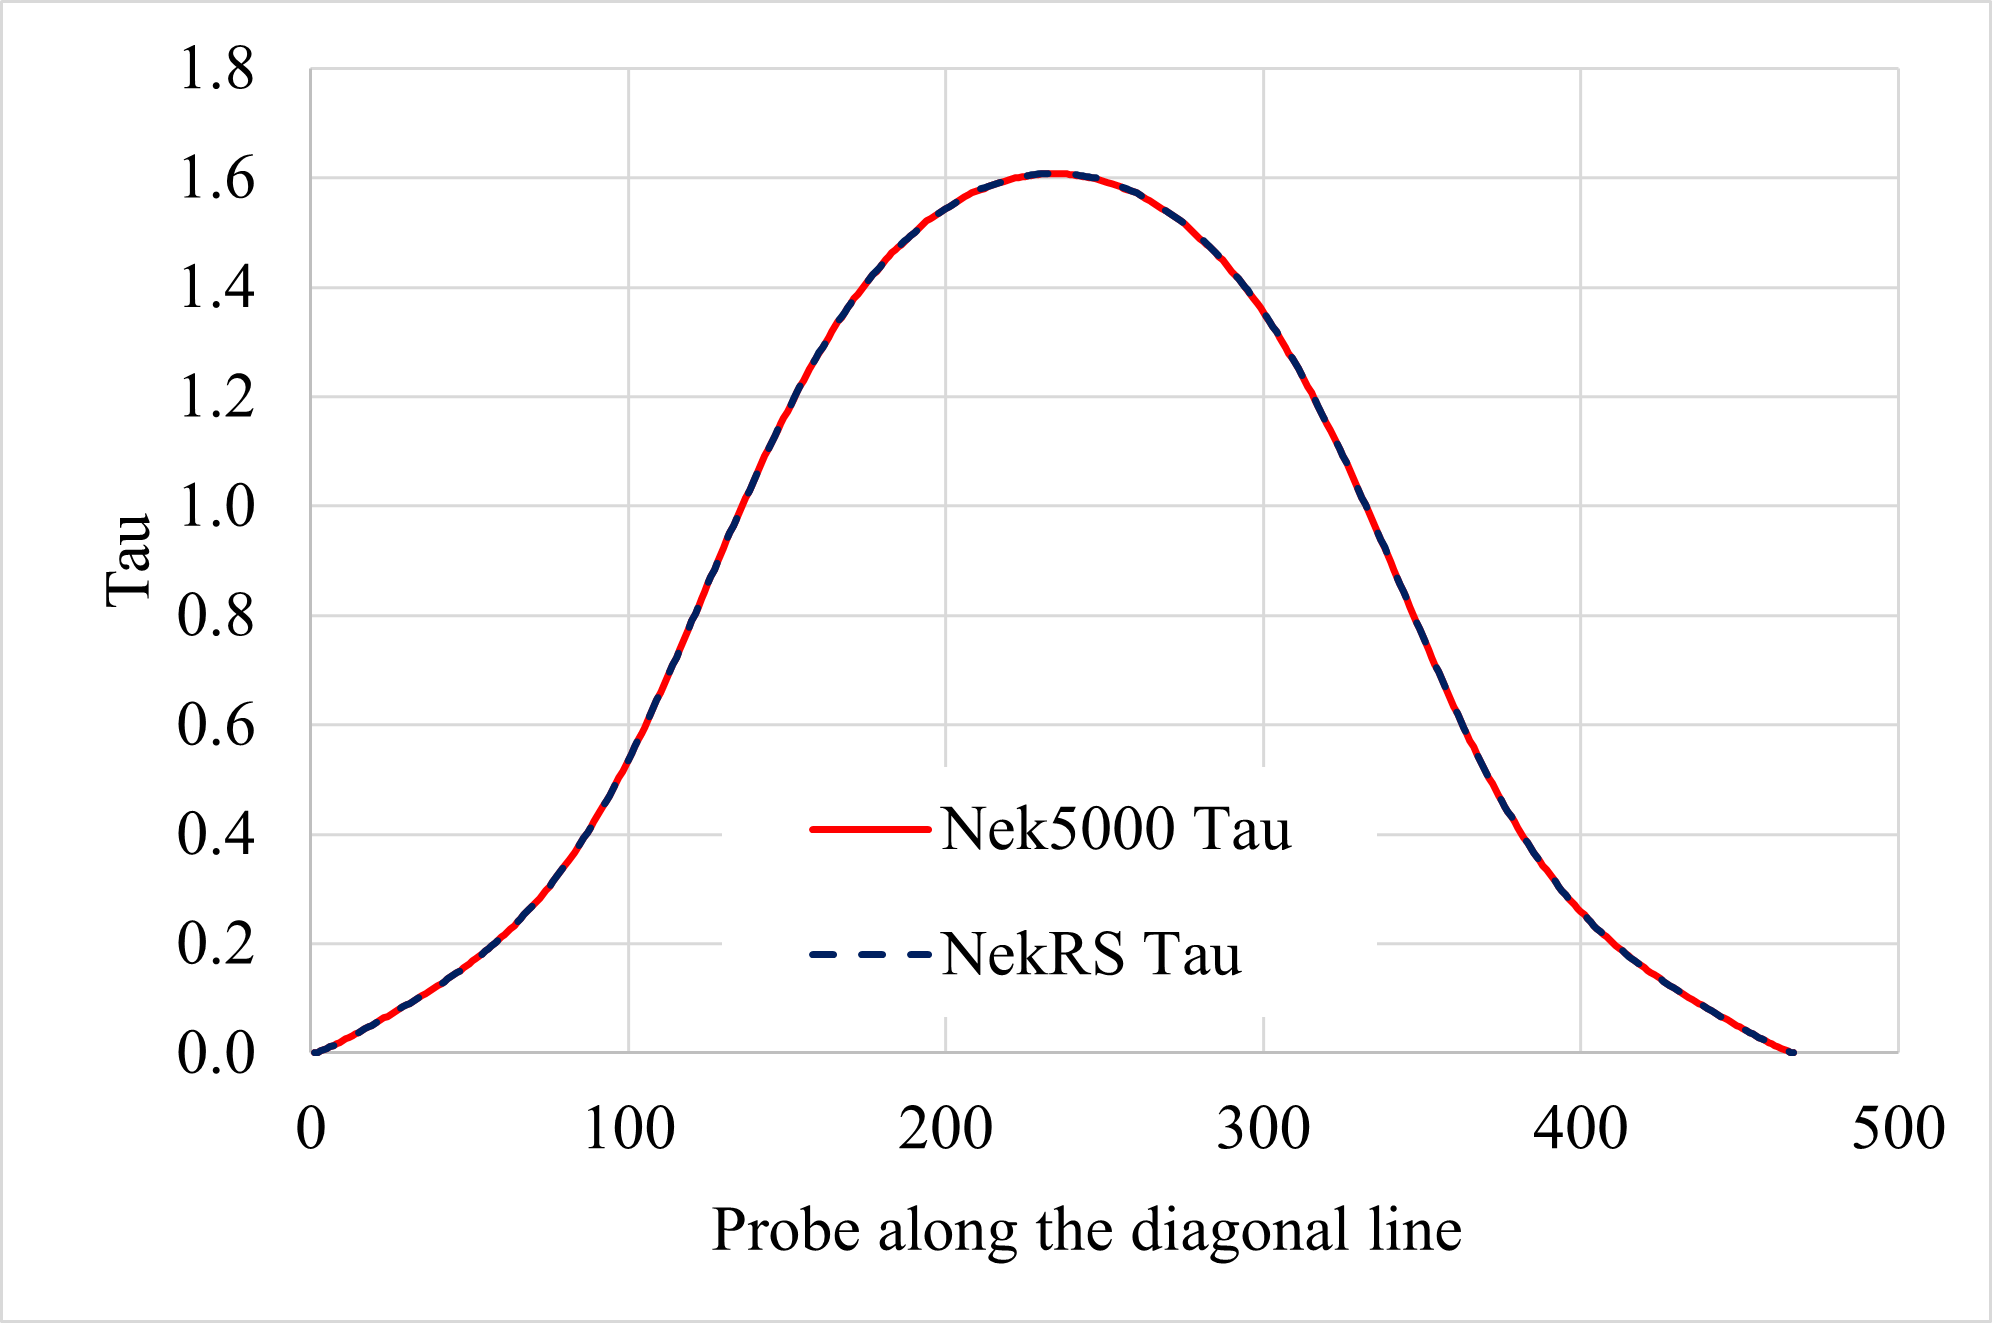
\includegraphics[width=0.5\textwidth]{./figures/tau_verification_bundle2x2.png}
\caption{Comparison of $\tau$ profile along the outlet diagonal line from Nek5000 and nekRS tests. }
\label{fig:tauplot}
\end{figure}